\section{Proposed work: Efficient clones}
\label{sec:clone}

We can build efficient clones on top of \rr.
Essentially, a rename is a clone with a delete.
\Rr swaps the sliced-out source and destination subtrees and uses \rd to
garbage collect the destination subtree.
Instead, clones can make the parent-to-child pointers in the source and
destination point to the same subtree and garbage collect the other destination
subtree separately.
With that, the source and destination share the content of the subtree.

We propose to explore the balance of sharing versus copying a cloned subtree
in a write-optimized dictionary.
Sharing a subtree saves space, however, when there is enough difference, it
might worth copying the subtree for better locality.
\bets only flush messages from parent to child when there are enough messages
in this flush.
At this point, we can break the sharing of the root of the subtree and keep
the sharing of the children.
In this way, \bets can gradually unshare the whole subtree.

The challenge is constructing multiple views of a single subtree.
Queries to the subtree following different root-to-subtree paths should fetch
the same value but with different keys.
Also, different root-to-subtree paths have different pending writes.

We also want to make \rr more efficient.
Currently, \rr locks the whole subtree while slicing from bottom up, forbidding
concurrent reads to the subtree.
Instead, \rr can use a top-down slicing, which unlocks parts of the subtree
during slicing.
Also, \rr completes with no delayed work, which doesn't fully utilize the
write-optimization of \bets.
Instead, we can have a message-based \rr that can be flushed down the \bet
gradually, like other messages in \bets.

\subsection{Smart pivots}

In \rr, both the source and the destination must be sliced out before the
pointer swing.
This approach is generic and applicable to other tree structures like B-trees.
However, it doesn't fit into the write-optimization of the \bet where
operations are inserted as messages and gradually flushed down in batches.

\subsubsection{\GOTO messages}

\begin{figure}
  \centering
  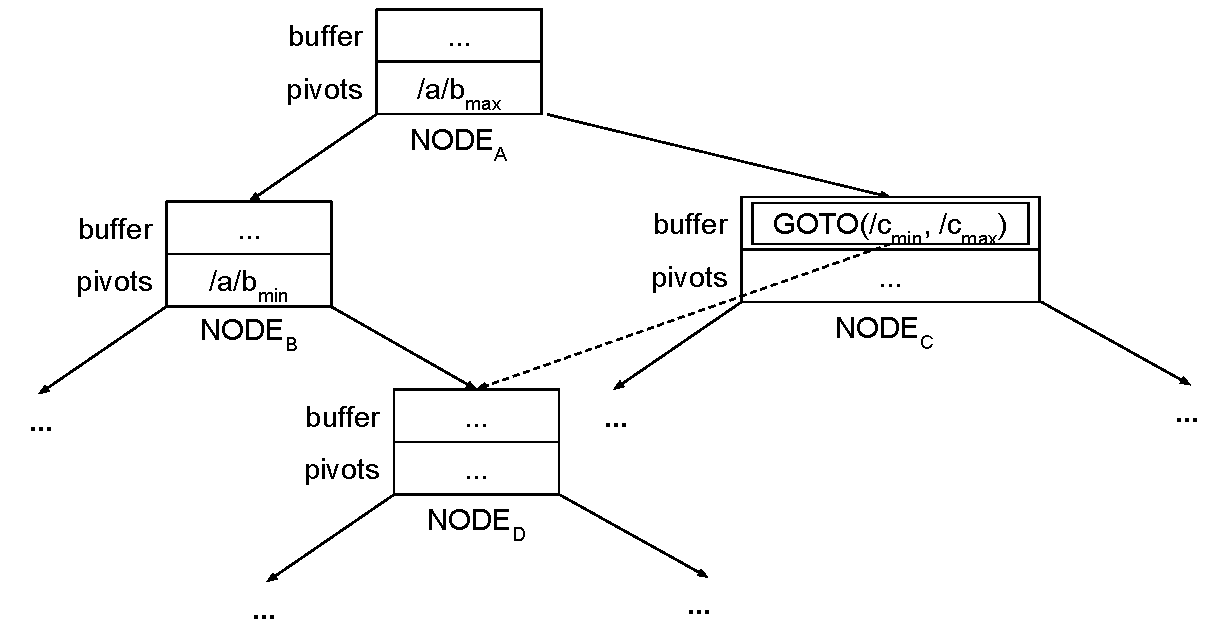
\includegraphics[width=.9\linewidth]{fig/goto}
  \caption{The \GOTO message directs queries of /c to another subtree.}
  \label{fig:goto}
\end{figure}

We can introduce a new type of message, \GOTO messages.
A \GOTO message has a range $(sp_l, sp_r)$ and points to the root of a subtree.
With \GOTO messages, after the source subtree is sliced out, a
\GOTO message, which specifies the destination range and the root of the
subtree, is injected to the root.

\GOTO messages would redirect queries.
Ordinarily, when a query for $key$ reaches one non-leaf node, it would find the
child whose range covers $key$ and continue to search that child.
However, if the query sees a \GOTO message in the node whose range covers $key$,
it would be redirected to the root of the subtree the \GOTO message points to.
Essentially, a \GOTO message acts as additional pivots in the node.

For example, ``clone /a/b to /c'' results in a \GOTO Message that covers
range $(/c_{min}, /c_{max})$ and points to the sliced out subtree whose range is
$(/a/b_{min}, /a/b_{max})$.
Figure~\ref{fig:goto} shows the \bet when the \GOTO message is flushed to
NODE$_C$.
Because keys in the \GOTO message are $c_{min}$ and $c_{max}$, the message is
flushed to the right child of NODE$_A$.
A query for /c/d searches NODE$_C$ after NODE$_A$, but when the query sees the
\GOTO message, it would then search NODE$_D$ instead of any child of NODE$_C$.

Like other messages, a \GOTO message is injected to the root of the \bet and
flushed down with other messages.
While a \GOTO message is flushed down the \bet, it can remove all old messages
in its range, like a \rd message.
Additionally, we can treat \rd messages as \GOTO messages that point to
nothing, thus generalizing range messages in the \bet.

To maintain the asymptotic IO cost for queries, all \GOTO messages in a node of
height $h$ must point to subtrees whose heights are less than $h$.
Otherwise, a query might have to search more than $O(tree\ height)$ nodes.
Therefore, a \GOTO message of height $h$ (the \GOTO message points to a subtree
of height $h$) must transform into something else before it is flushed to a node
of height $h$.

\begin{figure}
  \begin{subfigure}[b]{.45\textwidth}
  \centering
  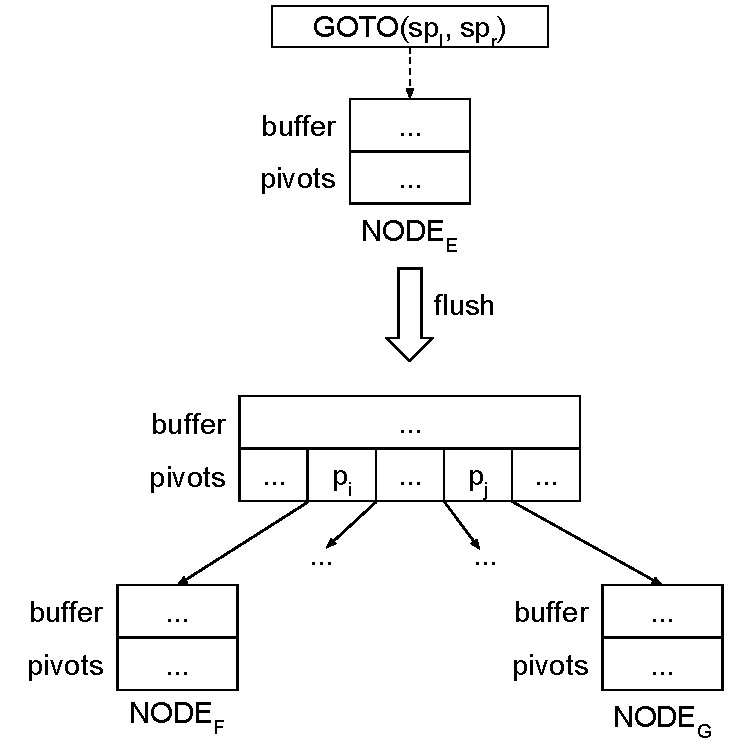
\includegraphics[width=.9\linewidth]{fig/flush-1}
  \caption{Before flushing.}
  \label{subfig:flush-1}
  \end{subfigure}
  \begin{subfigure}[b]{.45\textwidth}
  \centering
  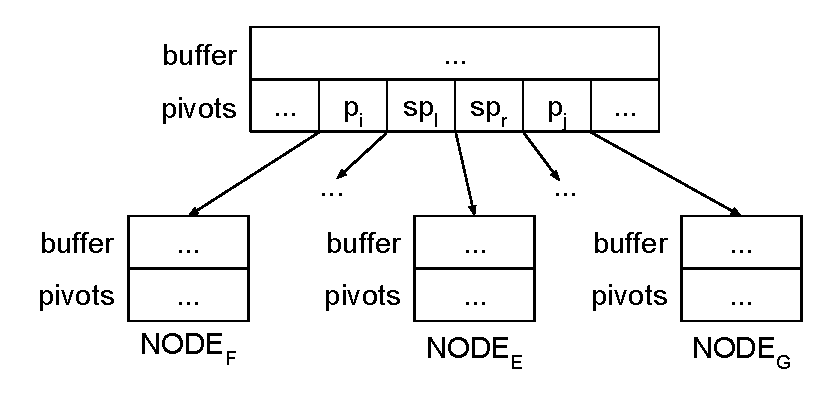
\includegraphics[width=.9\linewidth]{fig/flush-2}
  \caption{After flushing.}
  \label{subfig:flush-2}
  \end{subfigure}
  \caption{The \GOTO message of height $h$ transforms to real pivots
           when it is flushed to the node of height $h+1$
           ($p_0 < ... < p_i < sp_l < sp_r < p_j < p_n$).}
  \label{fig:flush}
\end{figure}

When a \GOTO message of height $h$ is flushed into a node of height $h+1$,
instead of injecting the message to the node buffer, we add two real pivots and
a child pointer to the node.
Figure~\ref{fig:flush} illustrates the process.
In Figure~\ref{subfig:flush-1}, the node contains pivots $p_0,...,p_n$,
the \GOTO message has range ($sp_l$, $sp_r$) and
$p_0 < ... < p_i < sp_l < sp_r < p_j < p_n$.
In Figure~\ref{subfig:flush-2}, pivots $p_{i+1}, ..., p_{j-1}$ are removed from
and $sp_l$ and $sp_r$ are added to the node.
The child pointer between $sp_l$ and $sp_r$ points to the subtree the \GOTO
message points to.
After that, the \GOTO message can be discarded.

In summary, \betrfs clones a file by slicing out the source subtree and putting
a \GOTO message to the root of the \bet.
The \bet flushes the \GOTO message down with other messages while garbage
collecting messages and subtrees.
When the \GOTO message reaches one level higher than the subtree, it transforms
to two pivots.

\subsubsection{\Spt messages}

\begin{figure}
  \centering
  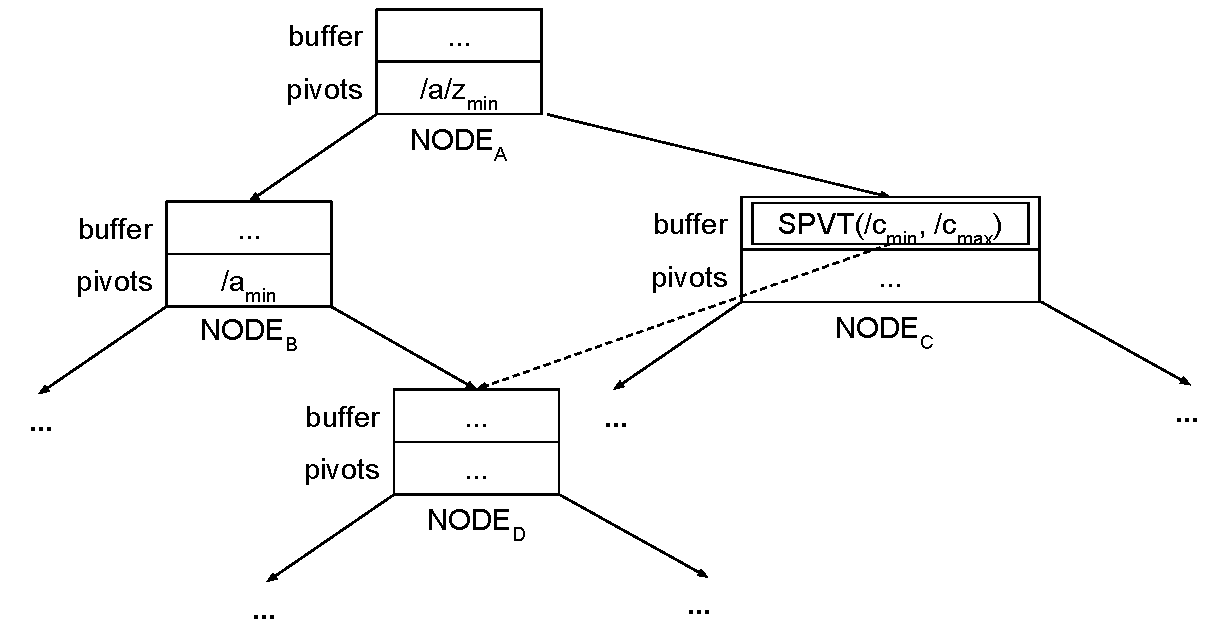
\includegraphics[width=.9\linewidth]{fig/spvt}
  \caption{The \spt message (SPVT) after ``clone /a/b to /c''. Note the subtree
           covers range ($/a_{min}$, $/a/z_{min}$), not
           ($/a/b_{min}$, $/a/b_{max}$).}
  \label{fig:spvt}
\end{figure}

Although \GOTO messages can be flushed down the \bet, they still require
slicing out the source and destination subtrees.
The source subtree needs to be sliced out because the \GOTO message has to point
to a subtree that is perfectly in range.
And when the \bet transform the \GOTO message, it needs to add pivots to the
node, which requires adjusting other children in the node to have the right
range.

All these problems are from the constraint that a subtree must cover the range
specified by its ancestors or the \GOTO message.
If this constraint can be removed, cloning can be further optimized.

Therefore, we introduce another type of messages, \spt.
Like \GOTO messages, a \spt message also has range $(sp_l, sp_r)$ but it can
point to a subtree whose range is larger than $(sp_l, sp_r)$.
This might break lifting because a large range can lift less.
Thus, the \spt message must also store what is lifted in the subtree.

Figure~\ref{fig:spvt} shows the \spt message of ``clone /a/b to /c''.
Note, the subtree is of range ($/a_{min}$, $/a/b_{min}$), whereas in
Figure~\ref{fig:goto}, the subtree must be of range
($/a/b_{min}$, $/a/b_{max}$).
The subtree may contain keys that are not in the range of the \spt mesasge,
for example, /a/a.
But queries can remember the range of \spt messages and ignore those keys.

Now, a \spt message can be injected immediately after the source LCA is found.
There is no need to slice the source subtree.
Also, \spt messages can be added when the \bet transforms the \spt message in
the destination.

\subsection{Garbage collection}

Since the introduction of \rd messages, garbage collection has long been
a problem in \betrfs.
If a subtree is completely in the range of a \rd message, unless \betrfs creates
some new entries with the same path, the \rd message might never be flushed
to the root of the subtree.
And the subtree will never be cleaned.

A background garbage collection thread can solve the problem.
If a \rd message covers a whole subtree, this thread should recycle all nodes
in the subtree.
The thread only needs to read the header of each node, which contains the block
numbers of its children and is much smaller than the whole node.

\Spt makes garbage collection more complicated.
A \spt message can hold a whole subtree before it becomes real pivots while
the \spt message only needs a small fraction of the subtree.
The garbage collection thread needs a way to figure out what parts of the
subtree are in use and what parts are not.

To this end, we can introduce \rrefc messages that, instead of incrementing
the reference count of the whole node, increment the reference count of a
certain key range.
When the garbage collection thread tries to clean up the whole subtree, it can
figure out which parts are still in use by \spt messages through
\rrefc messages.

Alternatively, the \rrefc information can be stored in the block table so
we don't need to write two copies of the node to remove the \rrefc message from
the node when the \spt message unshares the node.

\subsection{Preferential splitting}

A lot of work in both \rr and \spt attributes to handling fringe nodes, nodes
that contains both related and unrelated keys.
Therefore, it would be beneficial to reduce the number of fringe nodes.

The goal of preferential splitting is to reduce fringe nodes as much as
possible by carefully picking pivots in node splits.
Suppose range $(sp_l, sp_r)$ is cloned.
If one pivot in a node happens to be $sp_l$ or $sp_r$, this pivot already does
the work of separating keys and unrelated keys in the descendants of the node.
And there is no need to cut the \bet with $sp_l$ or $sp_r$ from this node on.

With preferential splitting, a leaf split lets \betrfs decide what the new
pivot is.
This split should not create unbalanced leaves, i.e., all resulting leaves
should be at least 1/4 of the full size.

A naive way would be comparing all keys in the range of [1/4, 3/4] of the leaf
and picking the pair of two adjacent keys that share the shortest common prefix.
But this scan can be costly.
For example, in \betrfs, a full leaf is 4MB and each key/value pair in
\texttt{meta\_db} is less than 200 Bytes, which means more than 10000 key
comparisons in preferential splitting..

We can do preferential splitting that only requires the reading two keys.
Because the shortest common prefix of adjacent keys is the same as the common
prefix of the smallest (at 1/4 of the leaf) and the largest (at 3/4 of the leaf)
candidate keys, we can construct a good pivot from these two keys.

Nonleaf splits can be viewed as promoting a pivot from the child to the parent.
Because the limit on the number of pivots in ft-index is 16, we can afford
one-to-one comparisons.

\subsection{Proposed evaluation}

We should focus on two aspects of \spt messages.
First, does \spt rename and clone fast enough?
Second, do \betrfs clones have good locality?
We can measure rename performance with the rename benchmark in our \rr work.
And we can modify this benchmark to measure clone performance.
We can measure locality by performing a file clone with subsequent writes to
two copies and then measuring the time to read two copies.
Besides, we can use Docker~\cite{docker} to benchmark clones in real
applications.
Docker is a container application that clones images for the starting contents.
Therefore, we can evaluate the common cases of file clones.

We should compare \betrfs with \spt to other cloning file systems.
Both Btrfs and XFS can do file clones.
ZFS and nilfs2 can create snapshots (immutable clones of the whole file system).
